
\section{some malicious things we'd like to stop}

\begin{frame}<1>[label=portalShouldnt]{things programs on portal shouldn't do}
    \begin{itemize}
    \item \myemph<2>{read other user's files}
    \item \myemph<3>{modify OS's memory}
    \item \myemph<3>{read other user's data in memory}
    \item \myemph<4>{hang the entire system}
    \end{itemize}
\end{frame}


\section{privileged instruction idea}
\againframe<2>{portalShouldnt}
\begin{frame}{privileged operation: problem}
\begin{itemize}
\item how can hardware (HW) plus operating system (OS) allow:
    \begin{itemize}
    \item read your own files from hard drive
    \end{itemize}
\item but disallow:
    \begin{itemize}
    \item read others files from hard drive
    \end{itemize}
\end{itemize}
\end{frame}

\begin{frame}{some ideas}
\begin{itemize}
\item<1-> OS tells HW `okay' parts of hard drive before running program code
    \begin{itemize}
    \item complex for hardware and for OS
    \end{itemize}
\item<2-> OS verifies your program's code can't do bad hard drive access 
    \begin{itemize}
    \item no work for HW, but complex for OS
    \item may require compiling differently to allow analysis
    \end{itemize}
\item<3-> \myemph<3>{OS tells HW to only allow OS-written code to access hard drive}
    \begin{itemize}
    \item that code can enforce only `good' accesses
    \item requires program code to call OS routines to access hard drive
    \item relatively simple for hardware 
    \end{itemize}
\end{itemize}
\end{frame}


\begin{frame}{kernel mode}
\begin{itemize}
\item extra one-bit register: ``are we in \textit{kernel mode}''
    \begin{itemize}
    \item other names: privileged mode, supervisor mode, \ldots
    \end{itemize}
\item not in kernel mode = \textit{user mode}
\vspace{.5cm}
\item certain operations only allowed in kernel mode
    \begin{itemize}
    \item \textit{privileged instructions}
    \end{itemize}
\item example: talking to any I/O device
\end{itemize}
\end{frame}

\begin{frame}{what runs in kernel mode?}
\begin{itemize}
\item system boots in kernel mode
\item OS switches to user mode to run program code
\vspace{.5cm}
\item next topic: when does system switch back to kernel mode?
    \begin{itemize}
    \item how does OS tell HW where the (trusted) OS code is?
    \end{itemize}
\end{itemize}
\end{frame}


\subsection{diagram with OS code in memory}
\usetikzlibrary{arrows.meta,decorations.pathreplacing,patterns}


\ifdefined\codeBoxA\else\newsavebox\codeBoxA\fi
\begin{lrbox}{\codeBoxA}
\lstset{language=C++,style=script}
\begin{lstlisting}
void readFromDiskInto(int diskLocation, char *dest) {
    ...
    runPrivilegedInstruction(...);
    ...
}
\end{lstlisting}
\end{lrbox}
\ifdefined\codeBoxB\else\newsavebox\codeBoxB\fi
\begin{lrbox}{\codeBoxB}
\lstset{language=C++,style=script}
\begin{lstlisting}
void readFileSafely(const char *name, char *dest) {
    if (canCurrentProgramCanAccessFile(name)) {
        readFromDiskInto(lookupFile(name), dest)
    }
}
\end{lstlisting}
\end{lrbox}

\begin{frame}[fragile,label=callOSDirectP]{calling the OS?}
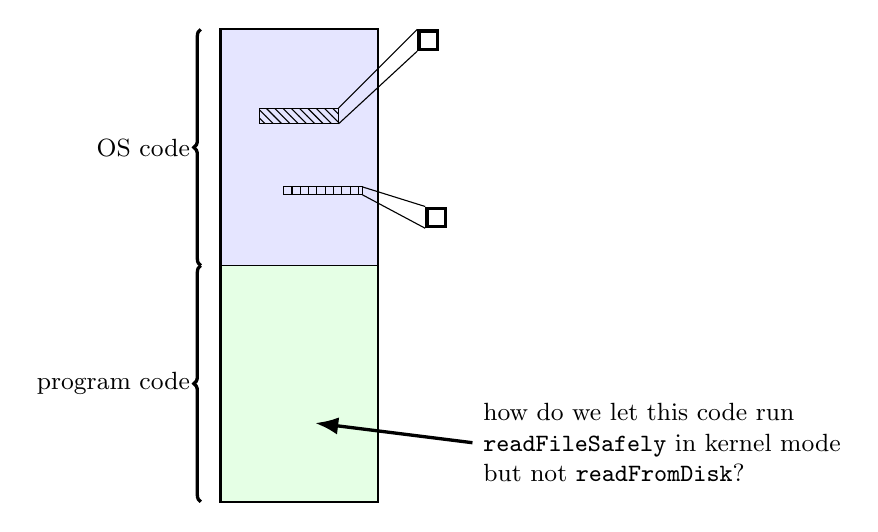
\begin{tikzpicture}
\draw[fill=blue!10] (0, 0) rectangle ++(2, -3);
\draw[fill=green!10] (0, -3) rectangle ++(2, -3);
\draw[thick] (0, 0) rectangle ++(2, -6);
\draw[very thick,decorate,decoration={brace,mirror}] (-.25, 0) -- ++(0, -3)
    node[midway,left] {OS code};
\draw[very thick,decorate,decoration={brace,mirror}] (-.25, -3) -- ++(0, -3)
    node[midway,left] {program code};
% FIXME: pointer to functions in OS
\draw[thin,pattern=north west lines] (0.5, -1) rectangle ++(1.0, -.2);
\draw[thin,pattern=vertical lines] (0.8, -2) rectangle ++(1.0, -.1);
\draw (1.5, -1.0) -- ++(1cm, 1cm) node[draw,very thick,anchor=north west,font=\tt\scriptsize] (readFromDiskInto) {
\usebox{\codeBoxA}
};
\draw (1.5, -1.2) -- (readFromDiskInto.south west);

\draw (1.8, -2.0) -- ++(.8cm, -.25cm) node[draw,very thick,anchor=north west,font=\tt\scriptsize] (readFileSafely) {
\usebox{\codeBoxB}
};
\draw (1.8, -2.1) -- (readFileSafely.south west);

\draw[very thick,Latex-] (1.2, -5) -- ++ (2cm, -.25cm) node[right,align=left] {
    how do we let this code run \\
    \texttt{readFileSafely} in kernel mode \\
    but not \texttt{readFromDisk}?
};
% FIXME: pointer to user code
\end{tikzpicture}
\end{frame}


\subsection{exception entry point}
\begin{frame}{controlled entry to kernel mode}
\begin{itemize}
\item OS specifies where to start executing code in kernel mode
    \begin{itemize}
    \item typically set at boot
    \item requires privileged instructions to change
    \end{itemize}
\item OS makes sure the code it says to start is ``safe''
    \begin{itemize}
    \item (hopefully)
    \item example: checks whether current program is allowed to read file before reading it
    \end{itemize}
\end{itemize}
\end{frame}


\subsection{system calls on Linux}
% FIXME import slides
\input{../kernel/sysCallLinux}

\subsection{system call wrappers}
\input{../kernel/syscallWrap}
% \begin{frame}{system call wrappers}
    \begin{itemize}
    \item can't write C code to generate syscall instruction
    \item solution: call ``wrapper'' function written in assembly
    \end{itemize}
\lstset{language=C++,style=smaller}
\begin{lstlisting}
\end{lstlsiting}
\end{frame}


\section{interlude: strace}
\input{../kernel/strace-hello}

\section{kernel + standard library}
% FIXME: diagram of kernel + standard library from whatisos
\usetikzlibrary{matrix}
\begin{frame}{hardware + system call interface}
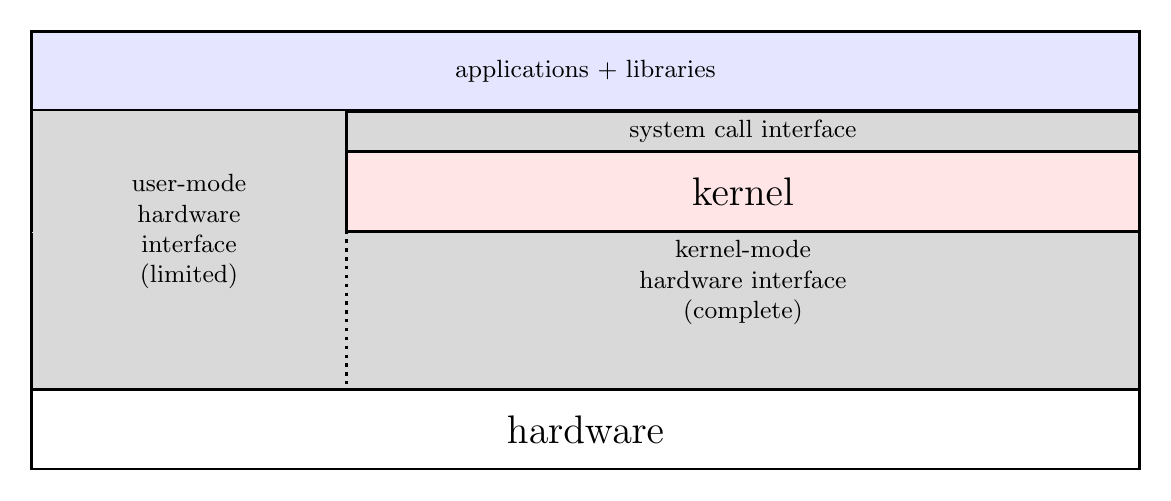
\begin{tikzpicture}
\tikzset{
    user/.style={fill=blue!10},
    iface/.style={fill=black!15},
    kernel/.style={fill=red!10},
    hardware/.style={},
}
% FIXME: show standard libraries/etc. can use HW directly
\matrix[matrix of nodes,
        inner sep=1pt, outer sep=0pt,
        row sep=-\pgflinewidth,
        column sep=-\pgflinewidth,
        nodes={draw,rectangle,inner sep=1pt,outer sep=0pt,thick,text width=14cm,align=center},
        ] {
    |[minimum height=1cm,alias=apps,user]| applications + libraries \\
    |[minimum height=0.5cm,alias=syscalls,iface,text width=10cm,xshift=2cm]| system call interface \\
    |[minimum height=1cm,alias=kernel,kernel,text width=10cm,xshift=2cm,font=\Large]| kernel \\
    |[minimum height=2cm,alias=hwIface,iface]| ~ \\
    |[minimum height=1cm,alias=hw,hardware,font=\Large]| hardware \\
};
\path[iface] (hwIface.north west) -- ++(4cm, 0cm) |- (apps.south west) |- (apps.south west) -- cycle;
\path[draw,very thick,black!15] ([xshift=4cm]hwIface.north west) -- (hwIface.north west);
\path[draw,thick] ([xshift=4cm]hwIface.north west) |- (apps.south west) |- (apps.south west) -- (hwIface.north west);
\path[draw,very thick,dotted] (kernel.south west) -- (kernel.south west |- hw.north);
\node[align=center] at ([xshift=2cm,yshift=0cm]hwIface.north west) {
    user-mode \\
    hardware \\
    interface \\
    (limited)
};
\node[anchor=north,align=center] at (kernel.south) {
    kernel-mode \\ hardware interface \\ (complete)
};
\end{tikzpicture}
\end{frame}

\begin{frame}{hardware + system call + library interface}
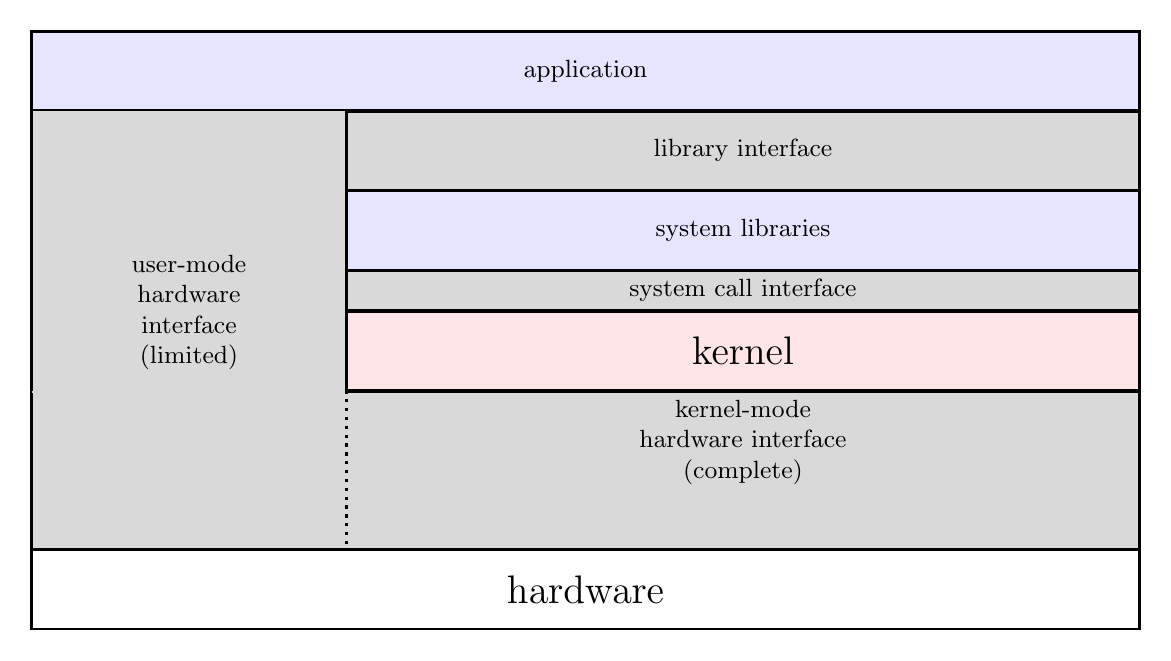
\begin{tikzpicture}
\tikzset{
    user/.style={fill=blue!10},
    iface/.style={fill=black!15},
    kernel/.style={fill=red!10},
    hardware/.style={},
}
% FIXME: show standard libraries/etc. can use HW directly
\matrix[matrix of nodes,
        inner sep=1pt, outer sep=0pt,
        row sep=-\pgflinewidth,
        column sep=-\pgflinewidth,
        nodes={draw,rectangle,inner sep=1pt,outer sep=0pt,thick,text width=14cm,align=center},
        ] {
    |[minimum height=1cm,alias=apps,user]| application \\
    |[minimum height=1cm,alias=syslibiface,iface,text width=10cm,xshift=2cm]| library interface \\
    |[minimum height=1cm,alias=stdlib,user,text width=10cm,xshift=2cm]| system libraries \\
    |[minimum height=0.5cm,alias=syscalls,iface,text width=10cm,xshift=2cm]| system call interface \\
    |[minimum height=1cm,alias=kernel,kernel,text width=10cm,xshift=2cm,font=\Large]| kernel \\
    |[minimum height=2cm,alias=hwIface,iface]| ~ \\
    |[minimum height=1cm,alias=hw,hardware,font=\Large]| hardware \\
};
\path[iface] (hwIface.north west) -- ++(4cm, 0cm) |- (stdlib.south west) |- (apps.south west) -- cycle;
\path[draw,very thick,black!15] ([xshift=4cm]hwIface.north west) -- (hwIface.north west);
\path[draw,thick] ([xshift=4cm]hwIface.north west) |- (stdlib.south west) |- (apps.south west) -- (hwIface.north west);
\path[draw,very thick,dotted] (kernel.south west) -- (kernel.south west |- hw.north);
\node[align=center] at ([xshift=2cm,yshift=1cm]hwIface.north west) {
    user-mode \\
    hardware \\
    interface \\
    (limited)
};
\node[anchor=north,align=center] at (kernel.south) {
    kernel-mode \\ hardware interface \\ (complete)
};
\end{tikzpicture}
\end{frame}


\input{../kernel/unix-design}

\section{memory protection}
\againframe<3>{portalShouldnt}

\subsubsection{exercise: expected behavior?}
\usetikzlibrary{positioning,shapes.multipart}

\begin{frame}<1-2>[label=memProtectQ]{memory protection}
\begin{itemize}
    \item modifying another program's memory?
\end{itemize}
\lstset{language=myasm,style=small,morekeywords={movq,.word}}
\begin{tabular}{l@{\hspace{.5cm}}|@{\hspace{.5cm}}l}
Program A & Program B \\ \hline
\lstinputlisting{../kernel/memprot-ex1.s} & \lstinputlisting{../kernel/memprot-ex2.s} \\ \hline
~ & ~ \\
\only<2>{result: {\tt \%rax} (in A) is \ldots} 
\only<3->{result: {\tt \%rax} (in A) is {\tt 42}} &
\only<4>{result: {\tt \%rax} (in B) is \ldots} 
\only<5->{result: \myemph{might crash}} \\
\only<3->{(with `normal' multiuser OSes)} \\
\end{tabular}

\begin{visibleenv}<2-5>
\small
A. 42 \hspace{1cm} B. 99 \hspace{1cm} C. 0x10000  \\
D. 42 or 99 (depending on timing/program layout/etc) \\
E. 42 or 99 or program might crash (depending on \ldots) \hspace{1cm} F. something else \\
\end{visibleenv}
\end{frame}

\iftoggle{heldback}{}{\againframe<3>{memProtectQ}}


\subsubsection{address spaces}
\input{../kernel/memProtectAddressSpaces}

\subsubsection{preview: shared memory}
\usetikzlibrary{arrows.meta,fit,positioning,shapes.multipart}
\begin{frame}[label=sharedMemAddr]{shared memory}
\begin{tikzpicture}
\tikzset{
    every node/.style={font=\small},
}
\node[align=center] (progAAddr) {Program A \\ addresses};
\node[below=1cm of progAAddr,align=center] (progBAddr) {Program B \\ addresses};
\node[draw, right=1cm of progAAddr,align=center] (translationA) { mapping \\ (set by OS) };
\node[draw, right=1cm of progBAddr,align=center] (translationB) { mapping \\ (set by OS) };
\node[draw,rectangle split, rectangle split parts=6, anchor=north west,label={north:real memory}] (mem) at ([xshift=1cm]translationA.north east) {
    \nodepart{one}
    Program A code 
    \nodepart{two}
    Program B code
    \nodepart{three}
    Program A data
    \nodepart{four}
    Program B data
    \nodepart{five}
    Shared code or data
    \nodepart{six}
    OS data
    \nodepart{seven}
    \ldots
};
\draw[-Latex,green,thick] (progAAddr) -- (translationA) (translationA.east) -- (mem.one west);
\draw[-Latex,green,thick] (translationA.east) -- (mem.three west);
\draw[-Latex,blue,thick] (progBAddr) -- (translationB) (translationB.east) -- (mem.two west);
\draw[-Latex,blue,thick] (translationB.east) -- (mem.four west);
\draw[-Latex,green,ultra thick,dotted] (translationA.east) -- (mem.six west);
\draw[-Latex,blue,ultra thick,dotted] (translationB.east) -- (mem.six west);
    \node[inner sep=0mm,fit=(mem.five split east) (mem.four split west),draw=red,ultra thick] {};
    \begin{pgfonlayer}{bg}
    \node[inner sep=0mm,fit=(mem.five split east) (mem.four split west),draw=red,fill=red!10,ultra thick] {};
    \end{pgfonlayer}
\draw[-Latex,red,ultra thick] (translationA.east) -- (mem.five west);
\draw[-Latex,red,ultra thick] (translationB.east) -- (mem.five west);
\end{tikzpicture}
\end{frame}

\begin{frame}[fragile,label=shmMmap]{one way to set shared memory on Linux}
\lstset{style=smaller,language=C++}
\begin{lstlisting}
/* regular file, OR: */
int fd = open("/tmp/somefile.dat", O_RDWR);
/* special in-memory file */
int fd = shm_open("/name", O_RDWR);
...
/* make file's data accessible as memory */
void *memory = mmap(NULL, size, PROT_READ | PROT_WRITE,
                    MAP_SHARED, fd, 0);
\end{lstlisting}
\begin{itemize}
    \item mmap: ``map'' a file's data into your memory
        \begin{itemize}
        \item if MAP\_SHARED: same data for everyone mapping the file
        \end{itemize}
    \item will discuss a bit more when we talk about virtual memory
    \item part of how Linux loads dynamically linked libraries
\end{itemize}
\end{frame}


\section{infinite loop}
\againframe<4>{portalShouldnt}

\begin{frame}{an infinite loop}
\lstinputlisting[language=C]{../kernel/loop.c}
\begin{itemize}
\item If I run this on a shared department machine, can you still use it? \\
\ldots if the machine only has one core?
\end{itemize}
\end{frame}

\begin{frame}{timing nothing}
\lstinputlisting[firstline=18,language=C]{../kernel/timedloop.c}
\begin{itemize}
\item same instructions --- \myemph{same difference} each time?
\end{itemize}
\end{frame}

\begin{frame}{doing nothing on a busy system}
    % FIXME: wider versions?
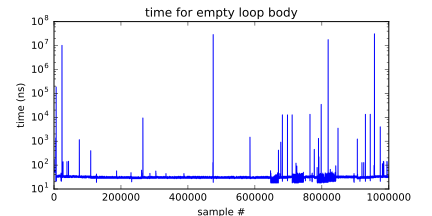
\includegraphics[width=\textwidth]{../kernel/empty-samples}
\end{frame}

\begin{frame}{doing nothing on a busy system}
\includegraphics[width=\textwidth]{../kernel/empty-samples-big-marked}
\end{frame}



\section{time multiplexing}
\usetikzlibrary{arrows.meta,patterns}

\begin{frame}\frametitle{time multiplexing}
\begin{tikzpicture}
\tikzset{
    prog1/.style={draw,fill=cyan!70},
    prog2/.style={draw,fill=green,visible on=<3->},
    prog3/.style={draw,fill=violet!30,visible on=<3->},
    proglabel/.style={font=\tt\scriptsize},
    labelprog1/.style={execute at begin node={\strut loop.exe}},
    labelprog2/.style={execute at begin node={\strut ssh.exe},visible on=<3->},
    labelprog3/.style={execute at begin node={\strut firefox.exe},visible on=<3->},
}
\begin{scope}[xscale=1.5,yscale=1]
\foreach \s/\e/\p [count=\x] in {0/2/1,2/3/2,3/5/3,5/6/1,6/7/2}{
    \draw[prog\p] (\s, 0) rectangle (\e, 1) coordinate[midway] (mid-\x);
    \node[anchor=center,proglabel,labelprog\p] at (mid-\x) {};
}
\end{scope}
\node[anchor=east] at (-0.25, 0.5) {processor:};
% FIXME: system
\begin{scope}[yscale=1,yshift=-2.5mm]
\draw[thick,-Latex] (1,0) node[left] {time} -- (10.5,0);
\end{scope}
\begin{visibleenv}<2->
    \begin{scope}[xscale=1.5]
    \draw[red,thick] (1.9,-.1) coordinate (firstStart) rectangle (2.0, 1.1);
    \draw[red,thick] (5.1,-.1) coordinate (lastEnd) rectangle (5.0, 1.1);
    \end{scope}
    \node[anchor=north west,font=\small\tt,align=left] (asmPre) at (0, -1) {
... \\
loop: ... \\
\hspace{1cm}... \\
\hspace{1cm}jmp loop \\
loop: ... \\
\hspace{1cm}...
    };
    \draw[red, ultra thick] ([xshift=-1cm,yshift=-.2cm]asmPre.south west) -- ([xshift=1cm,yshift=-.2cm]asmPre.south east) node [draw=none,midway,fill=white,
        inner sep=3pt] 
        {million cycle delay};
    \node[anchor=north west,font=\small\tt,align=left] (asmPost) at ([yshift=-.5cm]asmPre.south west) {
\hspace{1cm}... \\
\hspace{1cm}jmp loop \\
loop: ... \\
\hspace{1cm}...
    };
\end{visibleenv}
\end{tikzpicture}
\end{frame}



\subsection{context switching idea}
\input{../kernel/contextSwitchIntro}

\subsection{thread idea}
\begin{frame}{threads}
\begin{itemize}
\item thread = illusion of own processor
\vspace{.5cm}
\item own register values
\item own program counter value
\vspace{.5cm}
\item<2-> actual implementation: \\
    many threads sharing one processor
    \begin{itemize}
    \item problem: where are register/program counter values \\
        when thread not active on processor?
    \end{itemize}
\end{itemize}
\end{frame}


\subsection{context switches} 
\againframe<3>{timeMultiReally}
\usetikzlibrary{arrows.meta,calc,positioning,matrix,patterns}


\begin{frame}{OS and time multiplexing}
% FIXME: picture showing zoom of timeline
\begin{itemize}
\item starts running instead of normal program
    \begin{itemize}
    \item mechanism for this: \myemph{exceptions} (later)
    \end{itemize}
\item saves old program counter, registers somewhere
\item sets new registers, jumps to new program counter
\item called \myemph{context switch}
    \begin{itemize}
    \item saved information called \myemph{context}
    \end{itemize}
\end{itemize}
\end{frame}

\begin{frame}<2>[fragile,label=context]{context}
\begin{itemize}
\item all registers values
    \begin{itemize}
        \item \lstinline|%rax| \lstinline|%rbx|, \ldots, \myemph{\tt \%rsp}, \ldots
    \end{itemize}
\item condition codes
\item program counter
\item address space (map from program to real addresses)
\end{itemize}
\end{frame}

\begin{frame}[fragile,label=ctxtSwitchPseudo]{context switch pseudocode}
\lstset{
    style=small,
    language=myasm,
    morekeywords={copy_preexception_pc},
}
\begin{lstlisting}
context_switch(last, next):
  copy_preexception_pc last->pc
  mov rax,last->rax 
  mov rcx, last->rcx 
  mov rdx, last->rdx
  ...
  mov next->rdx, rdx
  mov next->rcx, rcx
  mov next->rax, rax
  jmp next->pc
\end{lstlisting}
\end{frame}

\tikzset{a/.style={fill=blue!30},b/.style={fill=green!30},>=Latex}
\newsavebox{\aContext}
\savebox{\aContext}{
\begin{tikzpicture}
\matrix[tight matrix,nodes={font=\small\tt,a}] (cpuState) {
    \%rax \& SF \\
    \%rbx \& ZF \\
    \%rcx \& PC \\
    \ldots \& \ldots \\
};
\end{tikzpicture}
}
\newsavebox{\bContext}
\savebox{\bContext}{
\begin{tikzpicture}
\matrix[tight matrix,nodes={font=\small\tt,b}] (cpuState) {
    \%rax \& SF \\
    \%rbx \& ZF \\
    \%rcx \& PC \\
    \ldots \& \ldots \\
};
\end{tikzpicture}
}


\begin{frame}{contexts (A running)}
\begin{tikzpicture}
\matrix[tight matrix,label={north:in CPU},nodes={font=\small\tt,a}] (cpuState) {
    \%rax \\
    \%rbx \\
    \%rcx \\
    \%rsp \\
    \ldots \\
    SF \\
    ZF \\
    PC \\
};

\matrix[tight matrix,right=3cm of cpuState, nodes={minimum height=2cm,text width=5cm,align=left},label={in Memory}] (memState) {
    |[a]| {Process A memory: \\ code, stack, etc.} \\
    |[b]| {Process B memory: \\ code, stack, etc.} \\
    |[fill=black!10]|{OS memory: \\ \usebox{\bContext} }\\
};
\draw[thick,dashed,->] (cpuState-4-1.east) -- (memState-1-1.west);
\draw[thick,dashed,->] (cpuState-8-1.east) -- (memState-1-1.west);
\end{tikzpicture}
\end{frame}

\begin{frame}{contexts (B running)}
\begin{tikzpicture}
\tikzset{a/.style={fill=blue!30},b/.style={fill=green!30}}
\matrix[tight matrix,label={north:in CPU},nodes={font=\small\tt,b}] (cpuState) {
    \%rax \\
    \%rbx \\
    \%rcx \\
    \%rsp \\
    \ldots \\
    SF \\
    ZF \\
    PC \\
};
\matrix[tight matrix,right=3cm of cpuState, nodes={minimum height=2cm,text width=5cm},label={north:in Memory}]
    (memState) {
    |[a]| {Process A memory: \\ code, stack, etc.} \\
    |[b]| {Process B memory: \\ code, stack, etc.} \\
    |[fill=black!10]| {OS memory: \\ \usebox{\aContext}} \\
};
\draw[thick,dashed,->] (cpuState-4-1.east) -- (memState-2-1.west);
\draw[thick,dashed,->] (cpuState-8-1.east) -- (memState-2-1.west);
\end{tikzpicture}
\end{frame}




\section{not just timers}
\input{../kernel/keyInTimeline}

\section{reasons for exceptions, generally}
\usetikzlibrary{decorations.pathreplacing}

\begin{frame}<0>[label=exceptTypesN]{types of exceptions}
\begin{itemize}
\item \tikzmark{trap bot}\myemph<2>{system calls}
    \begin{itemize}
    \item intentional --- ask OS to do something
    \end{itemize}
\item \tikzmark{fault bot}\myemph<3>{errors/events in programs}
    \begin{itemize}
    \item \myemph<8>{memory not in address space} (``Segmentation fault'')
    \item \myemph<9>{privileged instruction}
    \item \myemph<10>{divide by zero, invalid instruction}
    \item \tikzmark{invalid bot}\ldots
    \end{itemize}
\only<1-4>{(and more we'll talk about later)}
\item<5-> \tikzmark{int bot}\myemph<5>{external --- I/O, etc.}
    \begin{itemize}
    \item \myemph<6>{timer} --- configured by OS to run OS at certain time
    \item \myemph<7>{I/O devices} --- key presses, hard drives, networks, \ldots
    \item \tikzmark{abort bot}hardware is broken (e.g. memory parity error)
    \end{itemize}
\end{itemize}
\begin{tikzpicture}[overlay,remember picture]
    \coordinate (int top) at ([yshift=.6cm]pic cs:int bot);
    \coordinate (fault top) at ([yshift=.6cm]pic cs:fault bot);
    \coordinate (trap top) at ([yshift=.6cm]pic cs:trap bot);
    \coordinate (fault bot) at (pic cs:fault bot);
    \coordinate (over) at ([xshift=-4.5cm]current page.east);
    \coordinate (abort bot)  at (pic cs:abort bot);
    \coordinate (invalid bot)  at ([yshift=.6cm]pic cs:invalid bot);
    \begin{visibleenv}<5->
    \draw[very thick,decorate,decoration={brace}] (int top -| over) -- (abort bot -| over) 
        node[midway,right,font=\large] (async label) {\myemph<5>{asynchronous}};
        \node[anchor=north west,font=\small,align=left] at ([xshift=.15cm,yshift=.3cm]async label.south west) {
            not triggered by \\
            running program
        };
    \end{visibleenv}
    \begin{visibleenv}<4->
    \draw[very thick,decorate,decoration={brace}] (trap top -| over) -- (invalid bot -| over) 
        node[midway,right,font=\large] (sync label) {\myemph<4>{synchronous}};
        \node[anchor=north west,font=\small,align=left] at ([xshift=.15cm,yshift=.3cm]sync label.south west) {
            triggered by \\
            current program
        };
    \end{visibleenv}
\end{tikzpicture}
\end{frame}

\againframe<1>{exceptTypesN}

\subsection{aside: terms}
\begin{frame}{terms for exceptions}
    \begin{itemize}
    \item terms for exceptions aren't standardized
    \vspace{.5cm}
    \item our readings use one set of terms
    \begin{itemize}
        \item interrupts = externally-triggered
        \item faults = error/event in program
        \item trap = intentionally triggered
        \end{itemize}
    \item all these terms appear differently elsewhere
    \end{itemize}
\end{frame}


\section{exception table + dispatch}
\begin{frame}{exception implementation}
\begin{itemize}
\item detect condition (program error or external event)
\item save current value of PC somewhere
\item jump to \myemph{exception handler} (part of OS)
    \begin{itemize}
    \item jump done without program instruction to do so
    \end{itemize}
\end{itemize}
\end{frame}

\begin{frame}{exception implementation: notes}
\begin{itemize}
\item I describe a \myemph{simplified} version
\item real x86/x86-64 is a bit more complicated
    \begin{itemize}
    \item (mostly for historical reasons)
    \end{itemize}
\end{itemize}
\end{frame}




\section{exercise}
\begin{frame}{which of these require exceptions? context switches?}
    \begin{itemize}
    \item A. program calls a function in the standard library
    \item B. program writes a file to disk
    \item C. program A goes to sleep, letting program B run
    \item D. program exits
    \item E. program returns from one function to another function
    \item F. program pops a value from the stack
    \end{itemize}
\end{frame}

\iftoggle{heldback}{}{
\begin{frame}{which require exceptions [answers] (1)}
\begin{itemize}
    \item A. program calls a function in the standard library
        \begin{itemize}
        \item no (same as other functions in program; many standard library functions make no system calls (and do not otherwise trigger exceptions --- for example \texttt{strlen}, \texttt{pow}; also if we consider the calling of a function just the \texttt{call} instruction, then the library functions that do make system calls won't do so until later)
        \end{itemize}
    \item B. program writes a file to disk
        \begin{itemize}
        \item yes (requires kernel mode only operations)
        \end{itemize}
    \item C. program A goes to sleep, letting program B run
        \begin{itemize}
        \item yes (kernel mode usually required to change the address space to acess program B's memory)
        \end{itemize}
\end{itemize}
\end{frame}
\begin{frame}{which require exceptions [answer] (2)}
    \begin{itemize}
    \item D. program exits
        \begin{itemize}
        \item yes (requires switching to another program, which requires accessing OS data + other program's memory)
        \end{itemize}
    \item E. program returns from one function to another function
        \begin{itemize}
        \item no
        \end{itemize}
    \item F. program pops a value from the stack
        \begin{itemize}
        \item no
        \end{itemize}
    \end{itemize}
\end{frame}

\begin{frame}{which require context switches [answer]}
    \begin{itemize}
    \item no: A. program calls a function in the standard library
    \item no: B. program writes a file to disk
        \begin{itemize}
        \item (but might be done if program needs to wait for disk and other things could be run while it does)
        \end{itemize}
    \item yes: C. program A goes to sleep, letting program B run
    \item yes: D. program exits
    \item no: E. program returns from one function to another function
    \item no: F. program pops a value from the stack
    \end{itemize}
\end{frame}
}


\section{process}
\begin{frame}{The Process}
\begin{itemize}
\item \myemph{process} = thread(s) + address space
\item illusion of \myemph{dedicated machine}:
\begin{itemize}
\item thread = illusion of own CPU
\item (process could have multiple threads --- with independent registers)
\item address space = illusion of own memory
\end{itemize}
\end{itemize}
\end{frame}




\end{document}
